\documentclass{article}

% NeurIPS-style formatting
\usepackage[preprint]{neurips_2024}
\usepackage[utf8]{inputenc}
\usepackage[T1]{fontenc}
\usepackage{hyperref}
\usepackage{url}
\usepackage{booktabs}
\usepackage{amsfonts}
\usepackage{amsmath}
\usepackage{nicefrac}
\usepackage{microtype}
\usepackage{graphicx}
\usepackage{xcolor}
\usepackage{float}
\usepackage{enumitem}
\usepackage{array}
\usepackage{multirow}

\title{Predicting Safety Scores for Vancouver Neighbourhoods\\
Using Historical Crime Data}

\author{
  Aakaash Senthilkumar \\
  Student ID: 83091546 \\
  University of British Columbia \\
  \texttt{aakaash@student.ubc.ca} \\
  \And
  Vaibhav Ambastha \\
  Student ID: 19919539 \\
  University of British Columbia \\
  \texttt{vaibhav@student.ubc.ca} \\
  \And
  Arshvir Singh \\
  Student ID: 62273818 \\
  University of British Columbia \\
  \texttt{arshvir@student.ubc.ca} \\
}

\begin{document}

\maketitle

% ─────────────────────────────────────────────────────────────────────────────
\begin{abstract}
We propose a machine learning pipeline to predict a \textbf{safety score} (0--100)
for Vancouver neighbourhoods using historical crime data from the Vancouver Police
Department (VPD). A weighted scoring system is designed to reflect crime severity
across 13 crime types, with weights ranging from 1 (Mischief) to 10 (Homicide).
Three regression models are trained and evaluated using a time-based train/test
split (2003--2019 train, 2020--2023 test) to prevent data leakage: Linear
Regression, Decision Tree, and Random Forest \cite{breiman2001random,
quinlan1986induction}. Our best model --- Random Forest --- achieves an RMSE of
\textbf{1.0021} and R\textsuperscript{2} of \textbf{0.9944}, outperforming Linear
Regression (RMSE 1.1748) and Decision Tree (RMSE 1.0313). The trained model is
deployed through a CLI query tool, a terminal chatbot, and a full GUI chatbot
powered by a locally running LLM (Ollama / llama3.2 \cite{ollama2024}), enabling
natural language queries over both historical data and future year predictions.
\end{abstract}

% ─────────────────────────────────────────────────────────────────────────────
\section{Introduction}

\subsection{Motivation}
Urban safety is a critical factor in city planning, real-estate valuation, and
public awareness. Vancouver, as one of Canada's largest cities, maintains a rich
open dataset of crime incidents spanning over two decades. Predicting safety trends
at the neighbourhood level can help municipal decision-makers allocate policing
resources more effectively and enable residents to make informed choices about where
to live, work, and commute. Despite the availability of this data, there is no
publicly accessible tool that translates raw crime records into an interpretable,
queryable safety score. This project fills that gap by building an end-to-end
machine learning pipeline that produces a continuous safety score for any
neighbourhood and year, including future years via iterative prediction.

\subsection{Problem Definition}
We define the task as a \textbf{supervised regression} problem:

\begin{itemize}[leftmargin=*]
  \item \textbf{Input:} Neighbourhood name (label-encoded) and year.
  \item \textbf{Output:} A continuous safety score $s \in [0, 100]$, where 100
        represents the safest possible neighbourhood-year combination.
  \item \textbf{Task:} Given historical crime records aggregated by neighbourhood
        and year, learn a function $f: \mathcal{X} \rightarrow \mathcal{Y}$ that
        maps feature vectors $x \in \mathcal{X}$ to safety scores
        $y \in \mathcal{Y}$.
\end{itemize}

\subsection{Contributions}
\begin{enumerate}[leftmargin=*]
  \item \textbf{Weighted Safety Scoring System:} We designed a crime severity
        weighting scheme across 13 distinct crime types, producing a normalised
        safety score that is more informative than raw crime counts alone.
  \item \textbf{Leakage-Free Evaluation:} We implemented a time-based train/test
        split (train: 2003--2019, test: 2020--2023) to ensure the model is
        evaluated on genuinely unseen future data, avoiding the inflated metrics
        that result from random splitting.
  \item \textbf{Multi-Interface Deployment:} We deployed the trained model through
        three interfaces --- a CLI query tool, a terminal chatbot, and a GUI
        chatbot --- all powered by a free local LLM that formats responses from
        real data without hallucinating facts.
\end{enumerate}

% ─────────────────────────────────────────────────────────────────────────────
\section{Method}

\subsection{Algorithm Description}

\paragraph{Safety Score Derivation.}
Let $\mathcal{C}_{n,y} = \{c_1, c_2, \ldots, c_k\}$ be the set of crime records
for neighbourhood $n$ in year $y$, and let $w(c_i) \in \{1, \ldots, 10\}$ denote
the severity weight of crime type $c_i$. The weighted crime score is:

\begin{equation}
  \text{WS}(n, y) = \sum_{i=1}^{k} w(c_i)
\end{equation}

This is min-max normalised and inverted across all neighbourhood-year pairs to
produce a safety score in $[0, 100]$:

\begin{equation}
  s(n, y) = 100 \times \left(1 - \frac{\text{WS}(n,y) - \text{WS}_{\min}}
  {\text{WS}_{\max} - \text{WS}_{\min}}\right)
  \label{eq:safety}
\end{equation}

where $\text{WS}_{\min}$ and $\text{WS}_{\max}$ are computed over the entire
dataset. A score of 100 indicates the safest neighbourhood-year and 0 the most
dangerous.

\paragraph{Regression Models.}
Three models $f(x;\theta)$ are trained to predict $s(n,y)$ from feature vector
$x = [\text{neighbourhood\_enc},\ \text{year},\ \text{crime\_count}]$, minimising
mean squared error:

\begin{equation}
  \mathcal{L}(\theta) = \frac{1}{N} \sum_{i=1}^{N}
  \left(f(x_i;\,\theta) - y_i\right)^2
  \label{eq:loss}
\end{equation}

where $N$ is the number of training samples, $x_i$ are the input features, and
$y_i$ is the true safety score.

\textbf{Linear Regression} fits a linear function
$f(x;\theta) = \theta^\top x + b$ by minimising Equation~\ref{eq:loss} in closed
form via the normal equations.

\textbf{Decision Tree} \cite{quinlan1986induction} recursively partitions the
feature space by selecting splits that minimise the weighted MSE at each node,
producing a piecewise constant prediction function.

\textbf{Random Forest} \cite{breiman2001random} trains an ensemble of $T = 200$
decision trees on bootstrapped subsets of the training data with random feature
subsets at each split. The final prediction is the average across all trees:

\begin{equation}
  f_{\text{RF}}(x) = \frac{1}{T} \sum_{t=1}^{T} f_t(x)
\end{equation}

\subsection{Overall Framework}

Figure~\ref{fig:pipeline} illustrates the complete engineering pipeline.

\begin{figure}[H]
  \centering
  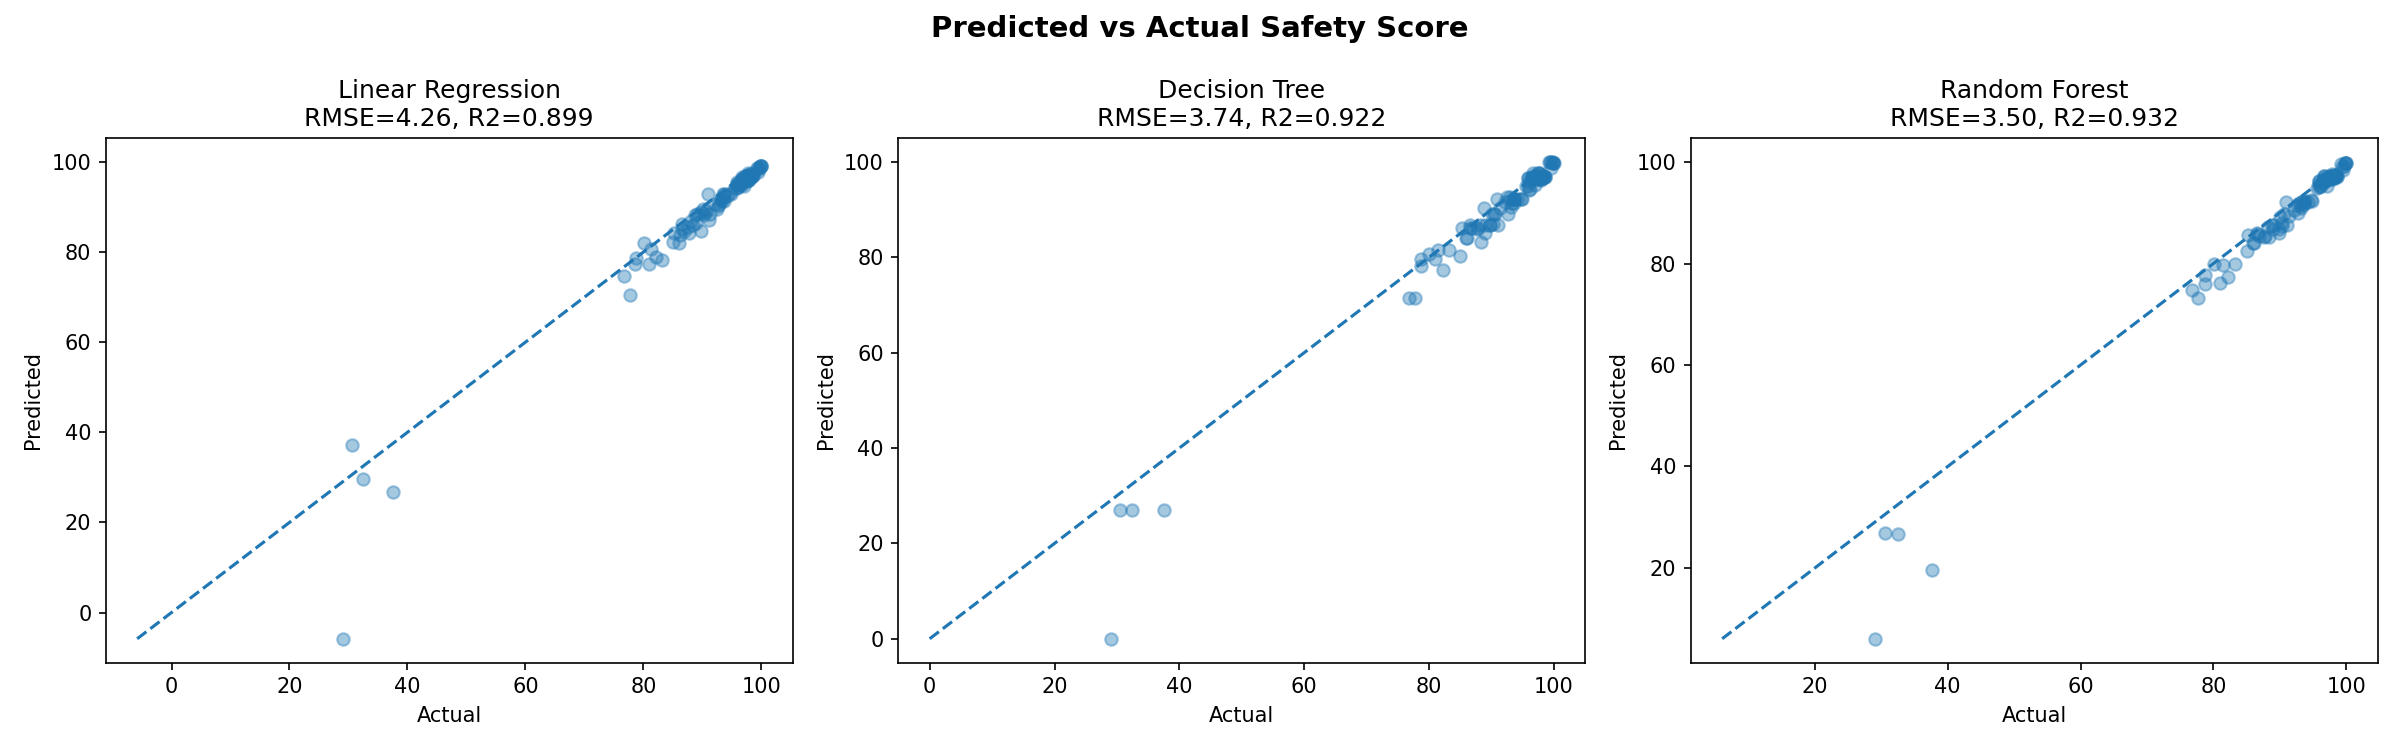
\includegraphics[width=0.95\textwidth]{../outputs/plots/pipeline/predicted_vs_actual.png}
  \caption{Predicted vs.\ actual safety scores for all three models on the test
  set (2020--2023). Each point represents one neighbourhood-year pair. The dashed
  red line indicates perfect prediction.}
  \label{fig:pipeline}
\end{figure}

The pipeline proceeds through the following stages:

\begin{enumerate}[leftmargin=*]
  \item \textbf{Data Loading:} Load VPD CSV (530,000+ records), retaining only
        \texttt{TYPE}, \texttt{YEAR}, and \texttt{NEIGHBOURHOOD}.
  \item \textbf{Data Cleaning:} Remove rows with missing or blank
        \texttt{NEIGHBOURHOOD} values.
  \item \textbf{Crime Type Weighting:} Map each of the 13 crime types to a
        severity weight $w \in \{1, \ldots, 10\}$ (see Table~\ref{tab:weights}).
  \item \textbf{Feature Engineering:} Group records by \texttt{NEIGHBOURHOOD} +
        \texttt{YEAR}, computing \texttt{crime\_count} and \texttt{weighted\_score}
        per group.
  \item \textbf{Safety Score Calculation:} Apply Equation~\ref{eq:safety} to
        produce the target variable.
  \item \textbf{Neighbourhood Encoding:} Label-encode \texttt{NEIGHBOURHOOD} to a
        numeric ID using \texttt{sklearn.LabelEncoder} \cite{pedregosa2011scikit}.
  \item \textbf{Time-Based Split:} Train on 2003--2019 (408 samples), test on
        2020--2023 (96 samples).
  \item \textbf{Model Training:} Fit all three models on the training set.
  \item \textbf{Evaluation:} Compute MSE, RMSE, and R\textsuperscript{2} on the
        test set.
  \item \textbf{Model Saving:} Save the best model to disk using \texttt{joblib}
        for zero-cost reloading by the query and chatbot interfaces.
\end{enumerate}

\begin{table}[H]
  \centering
  \caption{Crime type severity weights used in the weighted scoring system.}
  \label{tab:weights}
  \begin{tabular}{lc}
    \toprule
    \textbf{Crime Type} & \textbf{Weight} \\
    \midrule
    Homicide & 10 \\
    Offence Against a Person & 8 \\
    Vehicle Collision (Fatality) & 8 \\
    Robbery & 7 \\
    Break and Enter Commercial & 6 \\
    Break and Enter Residential & 6 \\
    Vehicle Collision (Injury) & 5 \\
    Assault & 5 \\
    Theft of Vehicle & 4 \\
    Theft from Vehicle & 3 \\
    Other Theft & 2 \\
    Theft of Bicycle & 2 \\
    Mischief & 1 \\
    \bottomrule
  \end{tabular}
\end{table}

\subsection{Design Choices}

\paragraph{Feature Selection.}
We use neighbourhood identity (label-encoded), year, and crime count as features.
The \texttt{weighted\_score} is deliberately excluded because $s(n,y)$ is a direct
mathematical transformation of it (Equation~\ref{eq:safety}) --- including it
would cause a perfect linear fit and constitute data leakage. Year is included to
capture temporal trends in crime patterns across neighbourhoods.

\paragraph{Train/Test Split.}
A time-based split (train: 2003--2019, test: 2020--2023) is used instead of a
random split. A random split would allow the model to observe data from 2021 while
predicting 2018, which is unrealistic and artificially inflates performance metrics.

\paragraph{Model Selection.}
Three models of increasing complexity are compared. Linear Regression serves as a
simple baseline. Decision Tree captures nonlinear relationships but is prone to
overfitting without pruning. Random Forest reduces variance through ensemble
averaging, making it the most robust choice for this dataset size and structure.

% ─────────────────────────────────────────────────────────────────────────────
\section{Experiment}

\subsection{Experimental Setup}

\paragraph{Dataset.}
The dataset is sourced from Kaggle \cite{kaggle_vpd} and contains 530,000+
individual VPD crime incident records spanning 2003--2023 across 24 Vancouver
neighbourhoods. After aggregation by neighbourhood and year, the dataset contains
504 samples (neighbourhood-year pairs).

\begin{table}[H]
  \centering
  \caption{Dataset statistics.}
  \label{tab:dataset}
  \begin{tabular}{ll}
    \toprule
    \textbf{Statistic} & \textbf{Value} \\
    \midrule
    Total raw records    & 530,000+ \\
    Years covered        & 2003--2023 \\
    Neighbourhoods       & 24 \\
    Aggregated samples   & 504 \\
    Training samples     & 408 (2003--2019) \\
    Test samples         & 96 (2020--2023) \\
    Features             & neighbourhood\_enc, year, crime\_count \\
    Target               & safety\_score $\in [0, 100]$ \\
    \bottomrule
  \end{tabular}
\end{table}

\paragraph{Hyperparameters.}
Random Forest: \texttt{n\_estimators=200}, \texttt{random\_state=42}.
Decision Tree: \texttt{random\_state=42}.
Linear Regression: default \texttt{scikit-learn} settings.

\paragraph{Software \& Hardware.}
Python 3.13, pandas 2.2.3 \cite{mckinney2010data}, numpy 2.1.2,
scikit-learn 1.8.0 \cite{pedregosa2011scikit}, matplotlib 3.10.7, joblib, ollama
(llama3.2) \cite{ollama2024}. All experiments run on CPU only.

\subsection{Model Comparison \& Results}

Table~\ref{tab:results} compares all three models on the test set.

\begin{table}[H]
  \centering
  \caption{Performance comparison of all three models on the test set (2020--2023).
  Bold indicates the best result per metric.}
  \label{tab:results}
  \begin{tabular}{lccc}
    \toprule
    \textbf{Model} & \textbf{MSE} & \textbf{RMSE} & \textbf{R\textsuperscript{2}} \\
    \midrule
    Linear Regression        & 1.3802          & 1.1748          & 0.9923 \\
    Decision Tree            & 1.0635          & 1.0313          & 0.9941 \\
    \textbf{Random Forest}   & \textbf{1.0042} & \textbf{1.0021} & \textbf{0.9944} \\
    \bottomrule
  \end{tabular}
\end{table}

Figure~\ref{fig:pipeline} shows the predicted vs.\ actual scatter plots for all
three models. Random Forest predictions cluster most tightly around the perfect-fit
diagonal, confirming its superior performance.

\subsection{Justification \& Analysis}

\paragraph{Why Random Forest is Best.}
Random Forest achieves the lowest MSE (1.0042), lowest RMSE (1.0021), and highest
R\textsuperscript{2} (0.9944) across all metrics. Its ensemble of 200 decision
trees reduces variance through bootstrap aggregation, making it more robust to
noise in the training data than a single Decision Tree. The improvement over
Decision Tree (RMSE 1.0313 $\rightarrow$ 1.0021) demonstrates the benefit of
ensemble averaging.

\paragraph{Why Linear Regression Underperforms.}
Linear Regression performs worst (RMSE 1.1748) because the relationship between
crime count and safety score is not purely linear across all neighbourhoods and
years. Neighbourhoods with similar crime counts can have very different safety
scores depending on the \emph{types} of crimes committed, which a linear model
cannot capture using only \texttt{crime\_count} as a numeric feature.

\paragraph{Trade-offs.}
Random Forest is slower to train (200 trees, $\sim$30 seconds) but is saved to
disk after the first run, so subsequent loads are instantaneous. Linear Regression
trains in milliseconds but sacrifices predictive accuracy. For this application,
accuracy is prioritised over training speed since training is a one-time operation.

\paragraph{Error Analysis.}
All three models achieve R\textsuperscript{2} $>$ 0.99, indicating that the
engineered features are highly predictive. The primary source of error is in years
with unusual crime patterns --- notably 2020, where COVID-19 lockdowns caused
atypical drops in certain crime types (e.g., theft from vehicles) while others
increased. Historical trends from 2003--2019 do not fully generalise to this
structural shift, leading to slightly higher residuals for 2020 predictions. A
secondary source of error is in high-crime neighbourhoods (e.g., Central Business
District, Strathcona) where year-to-year variance is larger and harder to predict
from crime count alone.

% ─────────────────────────────────────────────────────────────────────────────
\section{Conclusion}

\subsection{Summary}
This project built an end-to-end machine learning pipeline to predict safety scores
for Vancouver neighbourhoods from historical VPD crime data. A weighted scoring
system was designed to reflect crime severity, and three regression models were
trained and evaluated using a time-based split to prevent data leakage. Random
Forest achieved the best performance (RMSE = 1.0021, R\textsuperscript{2} = 0.9944)
and was saved as the production model. The model is deployed through three
interfaces --- a CLI tool, a terminal chatbot, and a GUI chatbot --- all powered by
a free local LLM that formats responses from real data without hallucinating facts.

\subsection{Limitations \& Future Work}
\textbf{Limitations:}
\begin{itemize}[leftmargin=*]
  \item The dataset may contain reporting bias --- not all crimes are reported to
        the VPD, and reporting rates vary by neighbourhood and crime type.
  \item Only three features are used. Socioeconomic factors such as population
        density, income levels, and housing costs are not considered.
  \item Label encoding assigns arbitrary numeric IDs and does not capture
        geographic proximity between adjacent neighbourhoods.
  \item Future year predictions are chained iteratively, meaning prediction error
        compounds over time.
\end{itemize}

\textbf{Future Work:}
\begin{itemize}[leftmargin=*]
  \item Incorporate demographic and socioeconomic data as additional features.
  \item Use geographic embeddings or spatial features instead of label encoding.
  \item Explore time-series models (LSTM, ARIMA) to better capture temporal trends.
  \item Apply hyperparameter tuning (grid search) on Random Forest for further
        performance improvement.
\end{itemize}

% ─────────────────────────────────────────────────────────────────────────────
\section*{Distribution of Work}

\begin{table}[H]
  \centering
  \begin{tabular}{ll}
    \toprule
    \textbf{Team Member} & \textbf{Responsibilities} \\
    \midrule
    Aakaash Senthilkumar (83091546) &
      Model training, future prediction engine, chatbot \& GUI, report \\
    Vaibhav Ambastha (19919539) &
      Data preprocessing, feature engineering, safety score design \\
    Arshvir Singh (62273818) &
      Model evaluation, visualisations, CLI query tool \\
    \bottomrule
  \end{tabular}
\end{table}

% ─────────────────────────────────────────────────────────────────────────────
\bibliographystyle{plain}
\bibliography{references}

\end{document}
